In this chapter we will provide and explain the concepts and terms that are used throughout this thesis.
We will cover the definitions of a GUI and GUI-Model as well as the basic terminology of a task tree, followed by
 information on alignment algorithms and substitution matrixes.
In the last section we describe the state of the art task tree generation based on n-grams\cite{harms2013}.


\section{GUI-Model}
\label{sec:foundationguiandguimodel}
A GUI-model is the structure of a graphical user interface. It consists of different elements those itself can have elements as children.
A GUI-model can be displayed as a tree. Figure \ref{fig:guimodel} shows a part of the GUI-model of the case study we will use in chapter \ref{chap:casestudy}.
\begin{figure}
	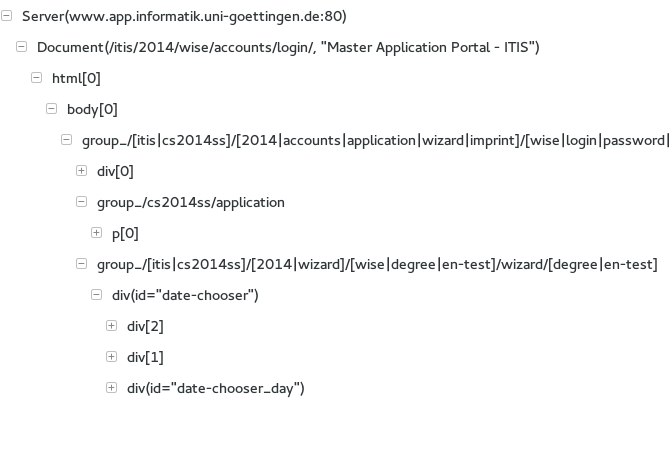
\includegraphics[width=\textwidth]{chapters/foundations/guimodel.png}
	\caption{Excerpt from a GUI Model of the website \texttt{www.app.informatik.uni-goettingen.de}}
	\label{fig:guimodel}
\end{figure}


\section{Task Tree Terminology}
\label{sec:foundationtasktreeterminology}
Harms et al.\cite{harms2013} have created a set of definitions and the respective vocabulary that help dealing with task trees.
We will adopt their definitions and summarize them in this section.

To understand tasks and task trees we have to look at how users interact with software.
Users, perfoming actions like clicking or typing, trigger so called events.
Those events consist of a type and a target.
The type describes the type of the action that triggered this event (e.g. onclick), the target describes the element in which the GUI the event occurred on.
The events a user creates can be traced, which is the basic step to gather data that is needed to generate task trees.
A trace is a list of events in the order they occurred. Table \ref{tab:trace} shows an example of such a trace.
All events in this list and their corresponding actions represent the users intention to achieve a goal, while using the software e.g. buying a book
in an online shop. From now on this goal is named task. This task can consist of several subtasks such as logging in or putting a book into the basket.
Each subtask itself can again contain further subtasks. From figure \ref{fig:booktree} one can see this results in a tree structure, a so called \textit{task tree}.

\begin{table}
\begin{center}
 \begin{tabular}{l|l|l}
	   Order & Type & Target \\
	 \hline
	 \hline
	   1. & Left mouse button click &  Textfield with ID username \\
	   2. & Text input "usr" &  Textfield with ID username \\
	   3. & Left mouse button click &  Textfield with ID username \\
	   4. & Text input "user" &  Textfield with ID username \\
	   5. &Left mouse button click &  Textfield with ID password \\
	   6. & Text input "" &  Textfield with ID password \\
	   7. &Left mouse button click &  Button with name "login" \\
	  \end{tabular}
  \end{center}
  \caption{Example for a trace of the login process of a user.\cite{harms2013}}
  \label{tab:trace}
  \end{table}

\begin{figure}
	\tikzstyle{every node}=[rectangle, draw=none, rounded corners=1mm,
        text centered, anchor=west, text=black, fill=blue!30]
\begin{tikzpicture}[%
  grow via three points={one child at (0.5,-0.7) and
  two children at (0.5,-0.7) and (0.5,-1.4)},
  edge from parent path={(\tikzparentnode.south) |- (\tikzchildnode.west)}]

\node {Buy a book} [-]
    child{
        node {Login}
        child{ node {Click on textfield "username"}}
        child{
            node {Enter user name into textfield "username"}
        }
        child{
            node {Click on textfield "password"}
        }
        child{
            node {Enter password  into textfield "password"}
        }
        child{
            node {Click on button "login"}
        }
    }
    child [missing] {}
    child [missing] {}
    child [missing] {}
    child [missing] {}
    child [missing] {}
    child{
        node {Search}
        child{
            node {Click into textfield "search"}
        }
        child{
            node {Type book name}
            child{
                node {Input "A"}
            }
            child{
                node {Input "B"}
            }
            child{
                node {Input "C"}
            }
        }
    child [missing] {}
    child [missing] {}
    child [missing] {}
        child{ node {Click on search button}}
    }
        child [missing] {}
        child [missing] {}
        child [missing] {}
        child [missing] {}
        child [missing] {}
        child [missing] {}
    child{ node {Basket}
        child{ node {...}}
    }
       child [missing] {}
    child{
        node {Order}
        child{ node {...}}
    }
;
\end{tikzpicture}

	\caption{Simplified and not complete visit of an online book shop as a task tree.}
	\label{fig:booktree}
\end{figure}

A task tree consists of three different kinds of nodes:
\begin{description}
	\item[Root node]\hfill\\ Represents the overall task which contains all subtasks, the user wants to achieve this goal by his actions/his input. In figure \ref{fig:booktree} the overall task is to buy books at an online shop.
	\item[Leaf nodes]\hfill\\ Actions (e.g. clicking, scrolling, textinput) cause an event (e.g. \textit{onclick} (click) or \textit{onchange} (textinput). The tasks at this level are called \textit{event tasks}. Event tasks do not have any further children. Some events tasks of \ref{fig:booktree} are for example Input A, Input B and Input C.
	\item[Intermediate nodes]\hfill\\ Subtasks which are steps towards the overall task. All tasks above the leave nodes are called non-event-tasks. In figure \ref{fig:booktree} the intermediate nodes are login, search, basket and order.
\end{description}
Another relevant point is that the order of the executed actions is important.
Therefore, this information has to be represented in the task tree as well.
For this, Harms et al. defined the so called \textit{temporal relationships} for all non-event-tasks.
There are four types of temporal relationships, each with different properties.
The \textit{sequence} temporal relationship dictates that children have to be executed in specific order to fulfil the task.
An \textit{iteration} can just have one child, which is executed once or several times.
Just one child of a \textit{selection} is allowed to be executed, whereas the one child of an \textit{optional} may or may not be executed.
Figure \ref{fig:exampletasktree} shows a task tree that represents a login procedure and contains all possible temporal relationships.
At last, Harms et al. differentiate between a task and an executed task, a task instance.
Figure \ref{fig:exampletaskinstancetree} shows the main differences between a task and its instance: \textit{selection} instances can have only one child with the task instance that was executed. \textit{Optional} instances have one child if the task was executed and none if the task was not executed. Instances of \textit{iterations} have as many children as often as the task was executed.
	\begin{figure}
		\tikzstyle{every node}=[rectangle, draw=none, rounded corners=1mm,
		        text centered, anchor=west, text=black, fill=blue!30]

		\begin{tikzpicture}[%
		  grow via three points={one child at (0.5,-0.7) and
		  two children at (0.5,-0.7) and (0.5,-1.4)},
		  edge from parent path={(\tikzparentnode.south) |- (\tikzchildnode.west)}]
		  \node {Sequence 1}
		    child { node {Iteration 1}
		      child { node {Selection 1}
		        child { node {Sequence 2}
				child { node {Click        on   textfield "username"}}
		          child { node {Enter user name    into textfield "username"}}
		      child [missing] {}
		          child [missing] {}
		    }
		        child [missing] {}
		    child [missing] {}
		        child { node {Sequence 3}
		          child { node {Click        on   textfield "password"}}
		          child { node {Enter password  into textfield "password"}}
		        }
		      }
		    }
		    child [missing] {}
		    child [missing] {}
		    child [missing] {}
		    child [missing] {}
		    child [missing] {}
		    child [missing] {}
		    child { node {Optional 1}
			    child { node {Iteration 2}
				child{ node{Scroll on page}}
			}
		    }
		    child [missing] {}
		    child [missing] {}
		    child { node {Click        on   button "login"}};
		    \end{tikzpicture}
		\caption{An example for a task tree with temporal relations. Adopted from Harms et al.\cite{harms2013}.}
		\label{fig:exampletasktree}
	\end{figure}
	\begin{figure}
		\tikzstyle{every node}=[rectangle, draw=none, rounded corners=1mm,
		        text centered, anchor=west, text=black, fill=green!30]

		\begin{tikzpicture}[%
		  grow via three points={one child at (0.5,-0.7) and
		  two children at (0.5,-0.7) and (0.5,-1.4)},
		  edge from parent path={(\tikzparentnode.south) |- (\tikzchildnode.west)}]
		  \node {Instance of Sequence 1}
		    child { node {Instance of Iteration 1}
		      child { node { Instance of Selection 1}
		        child { node { Instance of Sequence 2}
			  child { node {Click        on   textfield "username"}}
		          child { node {Enter user name    into textfield "username"}}
		          child [missing] {}
		          child [missing] {}
		        }
		      }
		      child [missing] {}
		      child [missing] {}
		      child [missing] {}
		      child { node { Instance of Selection 1}
			  child { node {Sequence 3}}
		          child { node {Click        on   textfield "password"}}
		          child { node {Enter password  into textfield "password"}}
		       }
	            }
		    child [missing] {}
		    child [missing] {}
		    child [missing] {}
		    child [missing] {}
		    child [missing] {}
		    child [missing] {}
		    child [missing] {}
		    child [missing] {}
		    child { node { Instance of Optional 1}}
		    child { node {Click        on   button "login"}};
		    \end{tikzpicture}
		\caption{An example for one task tree instance of the task tree in figure \ref{fig:exampletasktree} Adopted from Harms et al.\cite{harms2013}.}
		\label{fig:exampletaskinstancetree}
	\end{figure}

\section{State Of The Art Of Trace Based Task Tree Generation}
The current procedure to generate task trees\cite{harms2013} starts with iterating through the events in the traces and creates an event task instance for each.
Those event task instances are stored in the order they were triggered.  This structure is a so called \textit{user session}.

The user sessions used for task tree generation are available in a non-harmonized form,
meaning equal task instances may not have the same corresponding task assigned. TODO: Maybe write about the different levels of equality here?
The now following harmonization process sets the correct task to those task instances.
Fixing the issue of non-harmonized input data before starting any further steps is crucial since it reduces the number of occuring tasks and makes task instances
comparable by their tasks. Figure \ref{fig:nonharmonized} shows a non-harmonized user session, figure \ref{fig:harmonized} a session where the tasks of equal task instances have been set accordingly.

After the harmonization step follows the iteration detection, which detects any identical task instances that are direcly adjacent task instances in the user sessions. They occur if a user repeatedly does the same action (e.g. multiple clicks on the same button).
Once those subsequent instances have been detected, a new task of type iteration is generated.
We recall from the previous section that a task with a temporal relationship \textit{iteration} can just have one child, so the task of the detected iterated instance is added to this newly created iteration task.
Afterwards, this task is replaced in every other place it occurs as well.
In contradiction to the task, the iteration instance has, after the replacement, as many children of the instance as often the iterated instance occured.

The next part of the task tree generation algorithm is the sequence detection.
For this, the user sessions are scanned for identical subsequences. This is done with the help of a trie data structure.
The longest subsequence that occured most often is then added to a newly created \textit{sequence} task and again replaced in
all other user sessions as well. After that, the next most occuring subsequence is replaced. The minimal length of a subsequence is two.
If there is more than one subsequence with equal occurrence count, just the longest subsequence is replaced.
If both occurences match in count an length, Harms et al. just replace the subsequence occuring first in the ordered list.
Both steps, iteration detection and sequence detection are repeated until no more iterations or sequences are found.
Figure \ref{fig:exampletasktreeharms} shows an example of the first repetition of the task tree generation.

\begin{figure}
	\centering
	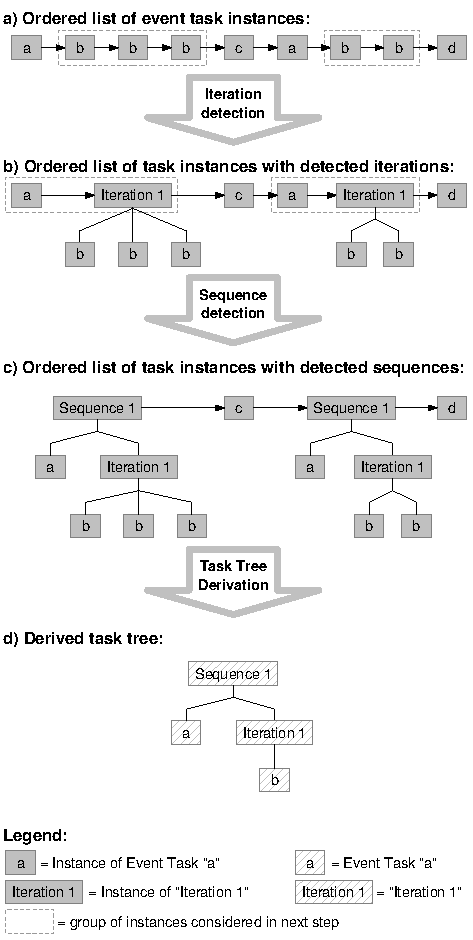
\includegraphics[scale=0.85]{chapters/foundations/TaskDetection.pdf}
	\caption{Example for one repetition of the iteration and sequence detection for task tree generation. Figure from Harms et al.}
	\label{fig:exampletasktreeharms}
\end{figure}

\begin{figure}

\[
\begin{array}{r|ccccc}
	Task & 1 & 2 & 3 & 4 & 5\\
	\hline
	Task instance & A & B & C & A & B\\
\end{array}
\]
\caption{Non-harmonized user session.}
\label{fig:nonharmonized}
\end{figure}

\begin{figure}
\[
\begin{array}{r|ccccc}
	Task & 1 & 2 & 3 & \textbf{1} & \textbf{2}\\
	\hline
	Task instance & A & B & C & A & B\\
\end{array}
\]
\caption{Harmonized user session. Task instance A now always has 1 as its task, task instance B always 2.}
\label{fig:harmonized}
\end{figure}

\section{Alignments}
\label{sec:alignments}
Alignments are a method in bioinformatics to compare strings or sequences of DNA/RNA/Amino acids and score their similarity.
It is a very basic method to find out if two sequences are related.
This is done by arranging those sequences in a way that similar elements of each sequence are aligned together. The biological background of this approach is that
both sequences have diverged from a common ancestor by a process of mutation and selection\cite{durbin1998}, hence still have common regions. Those regions are called conserved regions, meaning they were resistant to mutation.

In contrast to the persistent regions, differences between sequences can be explained by three processes: \textit{substitution}, which replaces one element with another,  \textit{deletion}, which removes an element and \textit{insertion}, which adds a new element to a sequence.
Both, insertion and deletion, produce a so called gap in the alignment, since the change just appeared in one of the two aligned sequences. Figure \ref{fig:alignmentbasic} illustrates all possible modifications.
Each modification can be scored individually but it is common practise to score substitutions with substitution matrixes and have a general gap penalty. The sum of all single scores is the score of the total alignment.
Alignment algorithms try to maximize this score.

\begin{figure}[h]
	\centering
	\begin{subfigure}[b]{0.3\textwidth}
	\begin{tabular}{c|cccc}
		1: &A&B&C&D\\
		2: &A&B&C&A\\
	\end{tabular}
	\caption{Substitution of D}
	\end{subfigure}
	\begin{subfigure}[b]{0.3\textwidth}
	\begin{tabular}{c|cccc}
		1:&A&B&C&D\\
		2:&A&B&-&D\\
	\end{tabular}
	\caption{Deletion of C}
	\end{subfigure}
	\begin{subfigure}[b]{0.3\textwidth}
	\begin{tabular}{c|cccc}
		1:&A&B&C&-\\
		2:&A&B&C&D\\
	\end{tabular}
	\caption{Insertion of D}
	\end{subfigure}
	\caption{Three possible modifications of sequence 2.}
	\label{fig:alignmentbasic}
\end{figure}

Alignments can be categorized into global and local alignments. Global alignment algorithms try to match one sequence with the other from start to end, whereas local alignment algorithms try to find the best alignment of subsequences.
A popular global alignment algorithm is the Needleman-Wunsch algorithm\cite{needleman1970}. For basic local alignments the common algorithm is from Smith and Waterman\cite{waterman1981}.

\section{Substitution Matrixes}
\label{sec:foundationsubstitutionmatrix}
In the last section we stated that alignment algorithms maximize the total alignment score. Therefore, the underlying scoring model has to be adjusted very carefully, since it practically determines the outcome of the algorithm.
There are usually two parameters which have to be set: the substitution score and the gap penalty.

\begin{definition}
	\item Let g be the gap penalty with $g>0$.
	\label{def:gappenalty}
\end{definition}

The gap penalty in its most basic version is a constant that has to be manually adjusted so that it fits the problem well.
A large gap penalty leads to less insertion and deletion occurrences and more substitutions.
This type of gap scoring is called linear affine gap penalty.
The total gap penalty is $n*g$ with n being the number of gaps and g the gap penalty constant.
There are different gap penalty models like a different g for opening a new gap and extending an already open gap.
In this thesis we will just use the linear affine gap penalty.

The substitution score is a representation of how similar two elements are. The more similar they are, the higher the score will be.
The score is usually stored in symmetric matrixes, where each cell represents how good or bad it is to substitute element a with element b.
The formal definition of the substitution matrix will follow in chapter approach.
%In biology
%	In Biology popular matrixes are generated from real DNA data (PAM, BLOSUM) (cite)
\begin{figure}
\centering
%\footnotesize
\scriptsize
\begin{verbatim}
      A    R    N    D    C    Q    E    G    H    I    L    K    M    F    P    S    T    W    Y    V
A    13    6    9    9    5    8    9   12    6    8    6    7    7    4   11   11   11    2    4    9
R     3   17    4    3    2    5    3    2    6    3    2    9    4    1    4    4    3    7    2    2
N     4    4    6    7    2    5    6    4    6    3    2    5    3    2    4    5    4    2    3    3
D     5    4    8   11    1    7   10    5    6    3    2    5    3    1    4    5    5    1    2    3
C     2    1    1    1   52    1    1    2    2    2    1    1    1    1    2    3    2    1    4    2
Q     3    5    5    6    1   10    7    3    7    2    3    5    3    1    4    3    3    1    2    3
E     5    4    7   11    1    9   12    5    6    3    2    5    3    1    4    5    5    1    2    3
G    12    5   10   10    4    7    9   27    5    5    4    6    5    3    8   11    9    2    3    7
H     2    5    5    4    2    7    4    2   15    2    2    3    2    2    3    3    2    2    3    2
I     3    2    2    2    2    2    2    2    2   10    6    2    6    5    2    3    4    1    3    9
L     6    4    4    3    2    6    4    3    5   15   34    4   20   13    5    4    6    6    7   13
K     6   18   10    8    2   10    8    5    8    5    4   24    9    2    6    8    8    4    3    5
M     1    1    1    1    0    1    1    1    1    2    3    2    6    2    1    1    1    1    1    2
F     2    1    2    1    1    1    1    1    3    5    6    1    4   32    1    2    2    4   20    3
P     7    5    5    4    3    5    4    5    5    3    3    4    3    2   20    6    5    1    2    4
S     9    6    8    7    7    6    7    9    6    5    4    7    5    3    9   10    9    4    4    6
T     8    5    6    6    4    5    5    6    4    6    4    6    5    3    6    8   11    2    3    6
W     0    2    0    0    0    0    0    0    1    0    1    0    0    1    0    1    0   55    1    0
Y     1    1    2    1    3    1    1    1    3    2    2    1    2   15    1    2    2    3   31    2
V     7    4    4    4    4    4    4    4    5    4   15   10    4   10    5    5    5   72    4   17
	\end{verbatim}
\normalsize
	\caption{An example for substitution matrixes: the PAM250 substitution matrix for amino acids\cite{dayhoff1978}. Note that biological substitution matrixes may not be symmetric.}
	\label{fig:submatexample}
\end{figure}
